\subsection{Traduction de la langue des signes}

\subsubsection{Vidéo de sourd en texte}

\begin{tcolorbox}[
  colback=gray!5,
  colframe=gray!40,
  arc=3mm,
  title={\textbf{Algorithme de traduction vidéo de sourd en texte}},
  fonttitle=\sffamily\bfseries
]
Pour traduire une vidéo de sourd en texte, on suit les étapes suivantes :

\begin{enumerate}
  \item Passage de la vidéo au modèle entraîné préalablement
  \item Paramétrage du modèle pour recevoir exactement 64 frames (succession d'images constituant la vidéo) 
  \item Chaque frame est redimensionnée à 224×224 pixels (largeur et hauteur)
  \item Extraction de toutes les frames de la vidéo
  \item Parcours des frames du début et envoi par groupes de 64 au modèle pour obtenir des prédictions
  \item Envoi des frames par lot de 64 en sautant 10 frames à chaque fois entre les lots
  \item Collecte de l'ensemble des prédictions faites par le modèle
  \item Reconstitution de la phrase dite dans la vidéo de sourd
\end{enumerate}

\textbf{Note:} Nous prenons les frames par bonds de 10 car par défaut 1 seconde de vidéo comporte 25 frames, 
et pour moins de 10 frames il n'y a pas vraiment de changement remarquable.
\end{tcolorbox}

\vspace{0.5cm}

\subsubsection{Texte en vidéo de sourd}

\begin{tcolorbox}[
  colback=gray!5,
  colframe=gray!40,
  arc=3mm,
  title={\textbf{Processus de traduction de texte en langue des signes}},
  fonttitle=\sffamily\bfseries
]
Pour traduire un texte en langage de sourd, le processus nécessite plusieurs étapes:

\begin{enumerate}
  \item Récupération du texte à partir de la source
  \item Analyse linguistique du texte pour déterminer les gestes correspondants
  \item Génération d'une séquence vidéo représentant les signes correspondant au texte
  \item Assemblage des mouvements pour former une communication fluide en langue des signes
\end{enumerate}

Cette technologie permet aux personnes malentendantes et sourdes d'accéder plus facilement à des contenus textuels qui seraient autrement difficiles à comprendre.
\end{tcolorbox}

\begin{figure}[H]
  \centering
  \begin{tcolorbox}[
    colback=white,
    colframe=gray!30,
    width=0.8\textwidth,
    arc=2mm,
    boxrule=0.5pt
  ]
    \centering
    \begin{minipage}{\linewidth}
      \centering
      \textbf{\Large Exemple de traduction}\\[0.3cm]
      \texttt{"Bonjour, comment allez-vous aujourd'hui?"}\\[0.3cm]
      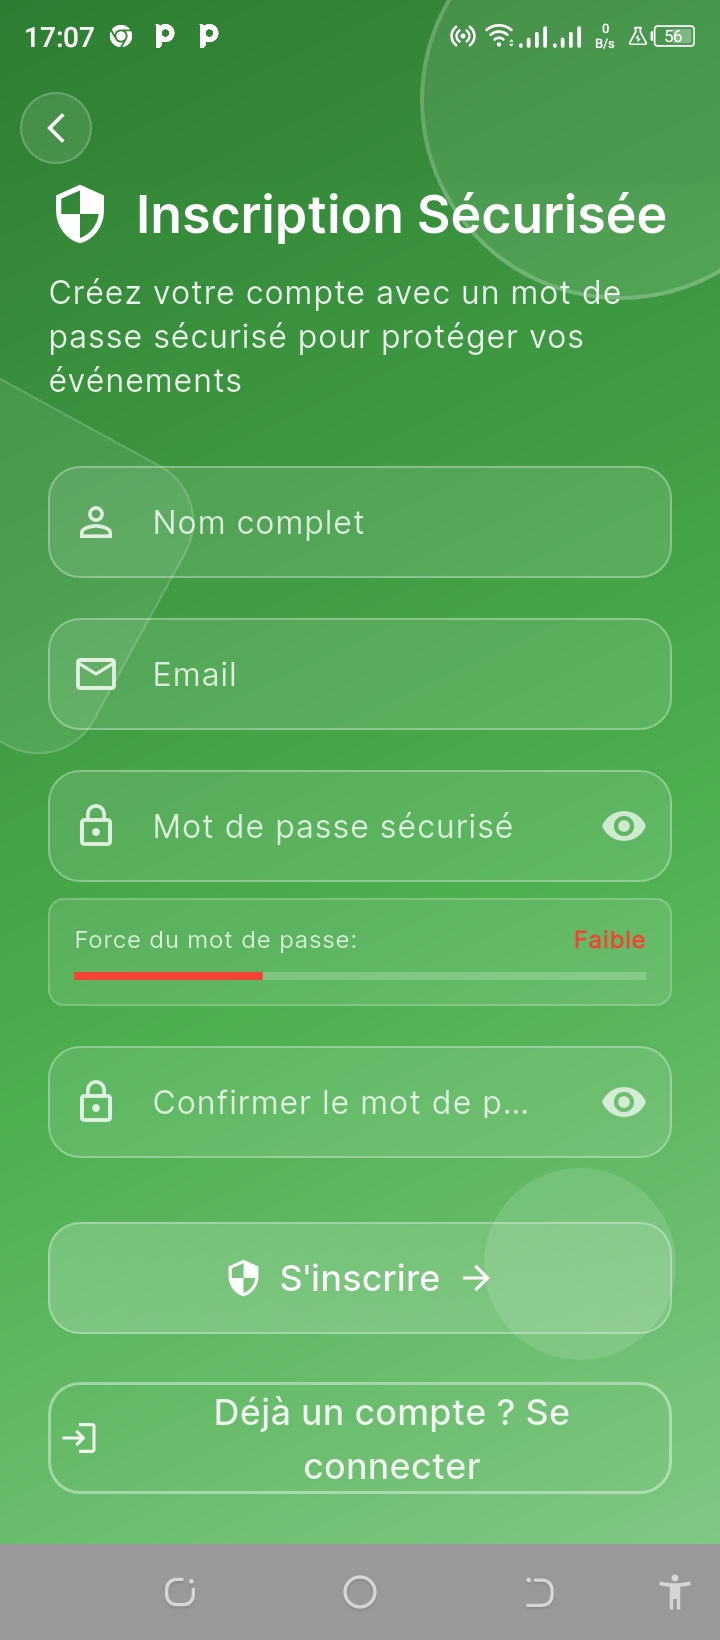
\includegraphics[width=0.7\linewidth]{images/page_inscription.jpg}\\
      \textit{Illustration de traduction en langue des signes}
    \end{minipage}
  \end{tcolorbox}
  \caption{Visualisation d'une traduction texte-langue des signes}
\end{figure}
